%template1.tex
%The following LaTeX source file represents the simplest kind of slide presentation; no overlays, no included graphics. Substitute your favorite style for ``pascal''. To create the PDF file template1.pdf, (1) be sure to use the prosper class, then (2) execute the command latex template1.tex, and (3) the command dvipdf template1.dvi.

%%%%%%%%%%%%%%%%%%%%%%%%%%%%%%% template1.tex %%%%%%%%%%%%%%%%%%%%%%%%%%%%%%%%%%%
\documentclass[a4paper,blends,pdf,colorBG,slideColor]{prosper}
% definitions for slides for CSC544
% Lutz Hamel, (c) 2007

\hypersetup{pdfpagemode=FullScreen}

\usepackage{amssymb}
\usepackage{latexsym}
\usepackage{amsmath}
%\usepackage[usenames]{color}
\usepackage{xypic}


\newcommand{\term}[1]{\ensuremath{\mbox{\bf #1}}}
\newcommand{\nonterm}[1]{\ensuremath{\mbox{#1}}}
\newcommand{\ifstmt}[3]{\ensuremath{{\bf if}\; {#1}\;{\bf then}\;{#2}\;{\bf else}\;{#3}\;\term{end}}}
\newcommand{\whilestmt}[2]{\ensuremath{{\bf while}\; {#1}\;{\bf do}\;{#2}\; \term{end}}}
\newcommand{\funcstmt}[3]{\ensuremath{{\bf fun}\; {#1}\; {\bf is}\; {#2} \; {\bf return}\; {#3}}}
\newcommand{\syntaxset}[1]{\ensuremath{\mbox{\bf #1}}}
\newcommand{\orbar}{\;|\;}
\newcommand{\bs}[1]{\begin{slide}{#1}\ptsize{8}}
\newcommand{\es}{\end{slide}}
\newcommand{\co}{\,\colon\;}
\newcommand{\pair}[2]{\ensuremath{\langle {#1}, {#2} \rangle}}
\newcommand{\encode}[1]{\ensuremath{\langle {#1} \rangle}}
\newcommand{\mytab}{\makebox[.15in]{}}
%\newcommand{\abs}[1]{{\mid{#1}\mid}}
\newcommand{\abs}[1]{{|{#1}|}}
\newcommand{\ol}[1]{\overline{#1}}

\newcommand{\qaccept}{\ensuremath{q_{\mbox{\tiny accept}}}}
\newcommand{\qreject}{\ensuremath{q_{\mbox{\tiny reject}}}}
\newcommand{\accept}{{\em accept}}
\newcommand{\reject}{{\em reject}}

\newcommand{\machine}[1]{
	\begin{quote}
	{#1}
	\end{quote}
	}

\newcommand{\fdef}[1]{
	\begin{center}
	\fbox{
	\begin{minipage}{3.5in}
	{\bf Definition:}
	{#1}
	\end{minipage}
	}
	\end{center}
	}

\newcommand{\ftheorem}[1]{
	\begin{center}
	\fbox{
	\begin{minipage}{3.5in}
	{\bf Theorem:}
	{#1}
	\end{minipage}
	}
	\end{center}
	}

\newcommand{\flemma}[1]{
	\begin{center}
	\fbox{
	\begin{minipage}{3.5in}
	{\bf Lemma:}
	{#1}
	\end{minipage}
	}
	\end{center}
	}


\newcommand{\fframe}[1]{
	\begin{center}
	\fbox{
	\begin{minipage}{3.5in}
	{#1}
	\end{minipage}
	}
	\end{center}
	}

\newcommand{\nframe}[1]{
	\begin{center}
	\begin{minipage}{3.5in}
	{#1}
	\end{minipage}
	\end{center}
	}

\begin{document}

\bs{Complexity Theory}
Up to now we investigated whether a problem is in principle solvable algorithmically,
that is, we asked the question whether a particular language is,
\begin{description}
\item[Decidable:] machine
halts on all inputs (total computable functions)
\item[Turing-Recognizable:] machine loops forever on some inputs (partially computable functions)
\end{description}
However, we did not investigate the cost of the computation itself - the amount of resources
the computation absorbs (time, space, {\em etc.})

In the following we discuss {\em time complexity} and {\em space complexity}.

Furthermore, we assume that we are dealing with total computable functions, that is,
the respective language is decidable.
\es

\bs{Time Complexity}

\fdef{Let $M$ be a deterministic TM that halts on all inputs.  The {\bf\em running time} or
{\bf\em time complexity} of $M$ is the function $f\co{\mathbb N} \rightarrow {\mathbb N}$,
where $f(n)$ is the {\em maximum number of steps} that $M$ uses on any input of length $n$.

If $f(n)$ is the running time of $M$, then we say that $M$ runs in time $f(n)$ and that $M$ is 
an $f(n)$ time TM.  Customarily we use $n$ to represent the length of the input.
}

Our time complexity analysis is called {\bf\em worst case analysis} because we only
consider the {\bf\em maximum number of steps} a machine uses on input $n$.
\es

\bs{Big-O Notation}
\vspace{.2in}
Asymptotic analysis or {\em big-O notation}.

\fdef{Let $f$ and $g$ be functions $f,g\co {\mathbb N} \rightarrow {\mathbb R}^+$.  Say that
\[f(n) =O(g(n))\] if positive integers $c$ and $n_0$ exist such that for every integer $n \ge n_0$,
\[
f(n) \le c\, g(n).
\]
When $f(n) = O(g(n))$ we say that $g(n)$ is an {\bf\em (asymptotic) upper bound} for $f(n)$.
}
\es

\bs{Big-O Notation}
\small
{\bf Example:} Let $f(n) = 5n^3 + 2n^2 + 22n + 6$, then only considering the highest order
term and disregarding all constants and coefficients we get
\[
f(n) = O(n^3).
\]
We can show that this satisfies our formal definition of asymptotic analysis by letting $c = 6$
and $n_0 = 10$.  Then for any $n > 10$ we have $f(n) \le 6 n^3$.
\begin{center}
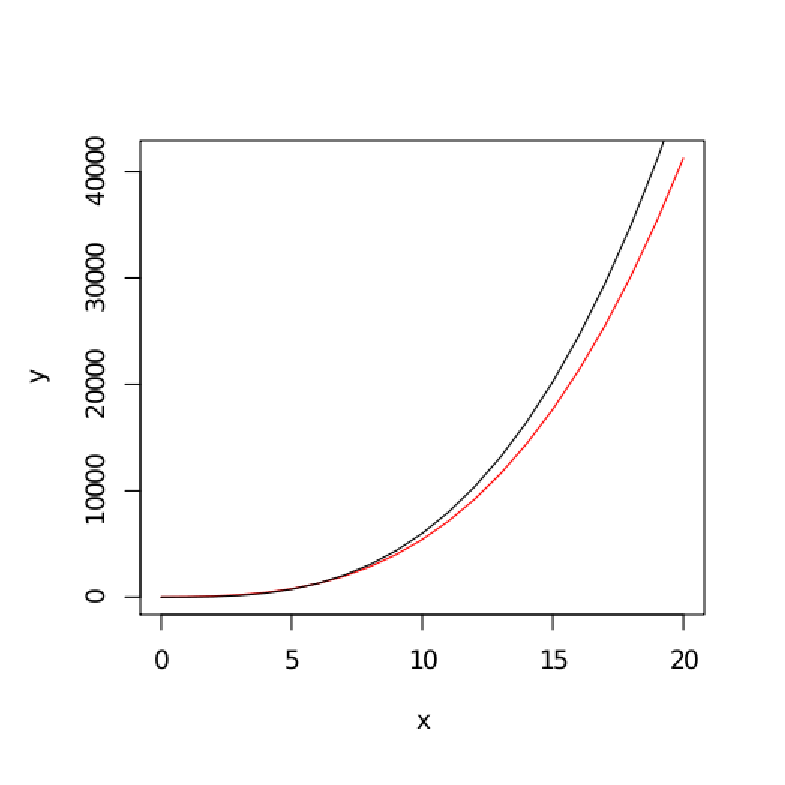
\includegraphics[height=50mm]{images/n3-complexity.eps}
\end{center}
\es

\bs{Big-O Notation}
{\bf Notes:}
\begin{itemize}
\item Let $f(n) = 3 n \log_2 n + 5n + 3$, then $f(n) = O(n\log n)$.  Notice that we dropped
the base subscript because $\log_b n = \frac{1}{\log_2 b}\log_2 n$ for any base $b$, that is
different logarithms are related to each other by a constant factor.
\item $f(n) = O(n^2) + O(n) \Rightarrow f(n) = O(n^2)$.
\item $f(n) = 2^{O(n)} \Rightarrow f(n) \le 2^{c n}$ for some $c$ and some value $n_0$ such
that $n > n_0$.
\end{itemize}

Bounds of the form $O(n^k)$ where $k > 0$ are called {\bf\em polynomial bounds}.
Bounds of the form $2^{O(n^k)}$ where $k > 0$ are called {\bf\em exponential bounds}.
\es

\bs{Analyzing Algorithms}
{\small
{\bf Example:} Given the decidable language
$
A = \{ o^k1^k | k \ge 0\}
$
and a TM $M_1$ that decides it, where
\begin{quote}
$M_1$ = "On input string $w$:
\begin{itemize}
\item[1.] Scan across the tape and \reject if a $0$ is found to the right
of a $1$.
\item[2.] Repeat the following if both $0$s and $1$s remain on the tape.
\item[3.]\mytab Scan across the tape, crossing off a single $0$ and a single $1$.
\item[4.] If neither $0$s nor $1$s remain on the tape \accept, otherwise \reject."
\end{itemize}
\end{quote}
To analyze the time complexity of this machine we analyze each stage separately:
\begin{description}
\item[stage 1:] The machine scans across the tape to verify that the input is of the
form $0^*1^*$.  Performing this scan uses $n$ steps where $n$ is the length of the input.
Repositioning the head to the beginning of the tape takes another $n$ steps.
Therefore, this stage takes $2n$ or $O(n)$ steps.
\item[stage 2,3:] Here the machine scans the input repeatedly.  Each scan takes $O(n)$
steps.  Since each scan crosses off two symbols at a time, at most $n/2$ scans
can occur.  That is $(n/2)O(n) = O(n^2)$.
\item[stage 4:] The machine makes a single scan over the input to decide whether to accept
or to reject - $O(n)$ steps.
\end{description}
Total time complexity of $M_1$ on input $n$ is $2O(n) + O(n^2) = O(n^2)$.
Can we find a faster algorithm or computational model?
}
\es

\bs{Analyzing Algorithms}
{\small
Consider the 2-tape machine $M_2$,
\begin{quote}
$M_2$ = "On input string $w$:
\begin{itemize}
\item[1.] Scan across tape $1$ and \reject if a $0$ is found to the right
of a $1$.
\item[2.] Scan across the $0$s on tape $1$ until the first $1$.  At the same time
copy the $0$s to tape $2$.
\item[3.] Scan across the $1$s on tape $1$ until the end of the input.
For each $1$ read on tape $1$ cross off a $0$ on tape $2$. If all $0$s
are crossed off before all $1$s are read, \reject.
\item[4.] If all $0$s have now been crossed off, \accept. If any $0$s remain, \reject."
\end{itemize}
\end{quote}
It is easy to see that each stage of this machine takes $O(n)$ steps - time complexity is $O(n)$
or linear!

{\bf Discussion:}  It is interesting to note that even though computability did not depend
on the precise model of computation chosen -- time complexity does! We saw that both our
machines, $M_1$ and $M_2$, decide the language $A$, but $M_1$ did it in time complexity
$O(n^2)$ and $M_2$ decided the language in time complexity $O(n)$.
}

\es
\end{document}
%%%%%%%%%%%%%%%%%%%%%%%%%%% end of template1.tex %%%%%%%%%%%%%%%%%%%%%%%%%%%%%%%%

